\documentclass[11pt,preprint]{elsarticle}

\usepackage{lmodern}
%%%% My spacing
\usepackage{setspace}
\setstretch{1.2}
\DeclareMathSizes{12}{14}{10}{10}

% Wrap around which gives all figures included the [H] command, or places it "here". This can be tedious to code in Rmarkdown.
\usepackage{float}
\let\origfigure\figure
\let\endorigfigure\endfigure
\renewenvironment{figure}[1][2] {
    \expandafter\origfigure\expandafter[H]
} {
    \endorigfigure
}

\let\origtable\table
\let\endorigtable\endtable
\renewenvironment{table}[1][2] {
    \expandafter\origtable\expandafter[H]
} {
    \endorigtable
}


\usepackage{ifxetex,ifluatex}
\usepackage{fixltx2e} % provides \textsubscript
\ifnum 0\ifxetex 1\fi\ifluatex 1\fi=0 % if pdftex
  \usepackage[T1]{fontenc}
  \usepackage[utf8]{inputenc}
\else % if luatex or xelatex
  \ifxetex
    \usepackage{mathspec}
    \usepackage{xltxtra,xunicode}
  \else
    \usepackage{fontspec}
  \fi
  \defaultfontfeatures{Mapping=tex-text,Scale=MatchLowercase}
  \newcommand{\euro}{€}
\fi

\usepackage{amssymb, amsmath, amsthm, amsfonts}

\def\bibsection{\section*{References}} %%% Make "References" appear before bibliography


\usepackage[numbers]{natbib}

\usepackage{longtable}
\usepackage[margin=2.3cm,bottom=2cm,top=2.5cm, includefoot]{geometry}
\usepackage{fancyhdr}
\usepackage[bottom, hang, flushmargin]{footmisc}
\usepackage{graphicx}
\numberwithin{equation}{section}
\numberwithin{figure}{section}
\numberwithin{table}{section}
\setlength{\parindent}{0cm}
\setlength{\parskip}{1.3ex plus 0.5ex minus 0.3ex}
\usepackage{textcomp}
\renewcommand{\headrulewidth}{0.2pt}
\renewcommand{\footrulewidth}{0.3pt}

\usepackage{array}
\newcolumntype{x}[1]{>{\centering\arraybackslash\hspace{0pt}}p{#1}}

%%%%  Remove the "preprint submitted to" part. Don't worry about this either, it just looks better without it:
\makeatletter
\def\ps@pprintTitle{%
  \let\@oddhead\@empty
  \let\@evenhead\@empty
  \let\@oddfoot\@empty
  \let\@evenfoot\@oddfoot
}
\makeatother

 \def\tightlist{} % This allows for subbullets!

\usepackage{hyperref}
\hypersetup{breaklinks=true,
            bookmarks=true,
            colorlinks=true,
            citecolor=blue,
            urlcolor=blue,
            linkcolor=blue,
            pdfborder={0 0 0}}


% The following packages allow huxtable to work:
\usepackage{siunitx}
\usepackage{multirow}
\usepackage{hhline}
\usepackage{calc}
\usepackage{tabularx}
\usepackage{booktabs}
\usepackage{caption}


\newenvironment{columns}[1][]{}{}

\newenvironment{column}[1]{\begin{minipage}{#1}\ignorespaces}{%
\end{minipage}
\ifhmode\unskip\fi
\aftergroup\useignorespacesandallpars}

\def\useignorespacesandallpars#1\ignorespaces\fi{%
#1\fi\ignorespacesandallpars}

\makeatletter
\def\ignorespacesandallpars{%
  \@ifnextchar\par
    {\expandafter\ignorespacesandallpars\@gobble}%
    {}%
}
\makeatother


% definitions for citeproc citations
\NewDocumentCommand\citeproctext{}{}
\NewDocumentCommand\citeproc{mm}{%
\href{\#cite.\detokenize{#1}}{#2}\nocite{#1}}

\makeatletter
% allow citations to break across lines
\let\@cite@ofmt\@firstofone
% avoid brackets around text for \cite:
\def\@biblabel#1{}
\def\@cite#1#2{{#1\if@tempswa , #2\fi}}
\makeatother
\newlength{\cslhangindent}
\setlength{\cslhangindent}{1.5em}
\newlength{\csllabelwidth}
\setlength{\csllabelwidth}{3em}
\newenvironment{CSLReferences}[2] % #1 hanging-indent, #2 entry-spacing
{\begin{list}{}{%
	\setlength{\itemindent}{0pt}
	\setlength{\leftmargin}{0pt}
	\setlength{\parsep}{0pt}
	% turn on hanging indent if param 1 is 1
	\ifodd #1
	\setlength{\leftmargin}{\cslhangindent}
	\setlength{\itemindent}{-1\cslhangindent}
	\fi
	% set entry spacing
	\setlength{\itemsep}{#2\baselineskip}}}
{\end{list}}

\usepackage{calc}
\newcommand{\CSLBlock}[1]{\hfill\break\parbox[t]{\linewidth}{\strut\ignorespaces#1\strut}}
\newcommand{\CSLLeftMargin}[1]{\parbox[t]{\csllabelwidth}{\strut#1\strut}}
\newcommand{\CSLRightInline}[1]{\parbox[t]{\linewidth - \csllabelwidth}{\strut#1\strut}}
\newcommand{\CSLIndent}[1]{\hspace{\cslhangindent}#1}


\urlstyle{same}  % don't use monospace font for urls
\setlength{\parindent}{0pt}
\setlength{\parskip}{6pt plus 2pt minus 1pt}
\setlength{\emergencystretch}{3em}  % prevent overfull lines
\setcounter{secnumdepth}{5}

%%% Use protect on footnotes to avoid problems with footnotes in titles
\let\rmarkdownfootnote\footnote%
\def\footnote{\protect\rmarkdownfootnote}
\IfFileExists{upquote.sty}{\usepackage{upquote}}{}

%%% Include extra packages specified by user

%%% Hard setting column skips for reports - this ensures greater consistency and control over the length settings in the document.
%% page layout
%% paragraphs
\setlength{\baselineskip}{12pt plus 0pt minus 0pt}
\setlength{\parskip}{12pt plus 0pt minus 0pt}
\setlength{\parindent}{0pt plus 0pt minus 0pt}
%% floats
\setlength{\floatsep}{12pt plus 0 pt minus 0pt}
\setlength{\textfloatsep}{20pt plus 0pt minus 0pt}
\setlength{\intextsep}{14pt plus 0pt minus 0pt}
\setlength{\dbltextfloatsep}{20pt plus 0pt minus 0pt}
\setlength{\dblfloatsep}{14pt plus 0pt minus 0pt}
%% maths
\setlength{\abovedisplayskip}{12pt plus 0pt minus 0pt}
\setlength{\belowdisplayskip}{12pt plus 0pt minus 0pt}
%% lists
\setlength{\topsep}{10pt plus 0pt minus 0pt}
\setlength{\partopsep}{3pt plus 0pt minus 0pt}
\setlength{\itemsep}{5pt plus 0pt minus 0pt}
\setlength{\labelsep}{8mm plus 0mm minus 0mm}
\setlength{\parsep}{\the\parskip}
\setlength{\listparindent}{\the\parindent}
%% verbatim
\setlength{\fboxsep}{5pt plus 0pt minus 0pt}



\begin{document}



\begin{frontmatter}  %

\title{Baby Names Persistence}

% Set to FALSE if wanting to remove title (for submission)




\author[Add1]{Tagishi Mashego}
\ead{tagishi@gmail.com}








\vspace{1cm}





\vspace{0.5cm}

\end{frontmatter}

\setcounter{footnote}{0}



%________________________
% Header and Footers
%%%%%%%%%%%%%%%%%%%%%%%%%%%%%%%%%
\pagestyle{fancy}
\chead{}
\rhead{}
\lfoot{}
\rfoot{\footnotesize Page \thepage}
\lhead{}
%\rfoot{\footnotesize Page \thepage } % "e.g. Page 2"
\cfoot{}

%\setlength\headheight{30pt}
%%%%%%%%%%%%%%%%%%%%%%%%%%%%%%%%%
%________________________

\headsep 35pt % So that header does not go over title




\section{Answer}\label{answer}

\subsection{Part 1}\label{part-1}

To help the New York-based agency make a well-informed decision about
naming its toy, I've included a Spearman correlation plot below. This
shows how the top 25 baby names persist over a three-year span, offering
insight into which names are likely to remain popular long enough for
the agency to capitalize on current naming trends and make the most
profits.

\begin{figure}[H]

{\centering 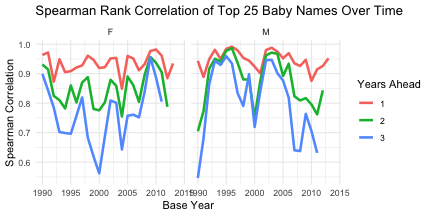
\includegraphics{Question1_files/figure-latex/Figure1-1} 

}

\caption{Correlation between each year's rankings and the next 3 years \label{Figure1}}\label{fig:Figure1}
\end{figure}

The Spearman correlation results in \ref{Figure1} show that the
strongest relationship is consistently between a given year and the year
immediately following it. This indicates that the top baby names remain
stable for at least one year. Further, as the years progress we see a
gradual decline , indicating that naming trends typically shift within a
few years. However, we see period of peaks and troughs indicating that
there are other reasons that affect the persistence of names. Lastly ,
the evidence indicates that male names tend to persist for a longer
duration.

A colleague of mine noted that there was a spike for the name Katina in
1974 , a character on the show ' Where The Heart Is'. To table below
adds robustness to \ref{Figure1} , testing whether the decay of trends
is inevitable irrespective of the size of the name spike.

\begin{table}[ht]
\centering
\begin{tabular}{rlrrr}
  \hline
Year & Gender & Offset & Future\_Year & Spearman \\ 
  \hline
1974 & F &   1 & 1975 & 0.94 \\ 
  1974 & F &   2 & 1976 & 0.83 \\ 
  1974 & F &   3 & 1977 & 0.63 \\ 
   \hline
\end{tabular}
\caption{Persistence of Female Names \label{tab1}} 
\end{table}

Table \ref{tab1} supports the findings from the Spearman correlation
analysis. Although there was a huge spike in the popularity of the name
Katina in 1974, the overall trend mirrors that observed for male names,
gradual decline over time. Nevertheless, there remains evidence of
moderate persistence in certain names.

\newpage

\subsection{Part 2}\label{part-2}

While the findings in Part 1 are informative, this section highlights
which character inspired names are most popular in the United States
which will provide further insight.

\begin{figure}[H]

{\centering 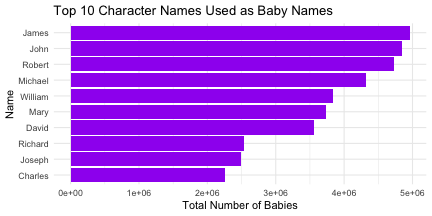
\includegraphics{Question1_files/figure-latex/Figure2-1} 

}

\caption{Popular Character Names \label{Figure2}}\label{fig:Figure2}
\end{figure}

The most popular character inspired name in the US over the duration of
the data is James , followed by John. What stands out to me immediately
is that these two names are also Bible names , given the deep religious
roots in America , perhaps we are overestimating the effect of the
characters in the naming trends in the US. In fact, most of the names in
the plot are bible names thus perhaps the agency ought to draw their
attention to that data. However, naming conventions have evolved over
time, with a noticeable shift toward more creative and unconventional
names. This prompts a closer examination of how the most popular names
have changed across different periods.

\begin{figure}[H]

{\centering 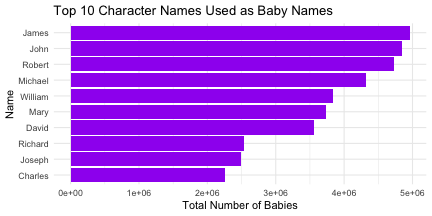
\includegraphics{Question1_files/figure-latex/Figure3-1} 

}

\caption{Name Trends \label{Figure3}}\label{fig:Figure3}
\end{figure}

Figure \ref{Figure3} shows a gradual decline in the number of babies
being named after these historically popular names. This trend coincides
with a broader cultural shift in which uniqueness is increasingly
valued, as reflected in modern naming conventions. Nevertheless, given
the strong biblical roots in the United States, the agency should still
consider drawing inspiration from traditional biblical names when naming
their toy.

\newpage

\section*{References}\label{references}
\addcontentsline{toc}{section}{References}

\phantomsection\label{refs}
\begin{CSLReferences}{1}{1}
\bibitem[\citeproctext]{ref-Texevier}
Katzke, N.F. 2017. \emph{{Texevier}: {P}ackage to create elsevier
templates for rmarkdown}. Stellenbosch, South Africa: Bureau for
Economic Research.

\end{CSLReferences}

\section*{Appendix}\label{appendix}
\addcontentsline{toc}{section}{Appendix}

\subsection*{Appendix A}\label{appendix-a}
\addcontentsline{toc}{subsection}{Appendix A}

Some appendix information here

\subsection*{Appendix B}\label{appendix-b}
\addcontentsline{toc}{subsection}{Appendix B}

Katzke (\citeproc{ref-Texevier}{2017})

\bibliography{Tex/ref}





\end{document}
